\documentclass[10pt,twocolumn]{article}
\usepackage{amsmath}
\usepackage[ruled,vlined]{algorithm2e}
\usepackage{amssymb}
\usepackage{xeCJK}
\usepackage{epstopdf}
\usepackage{hyperref}
\renewcommand\figurename{\hei 图}
\newCJKfontfamily\hei{Heiti SC}
\newCJKfontfamily\fs{FangSong}
\setCJKmainfont{FZShuSong-Z01S}
\setlength{\parindent}{2em}
\columnsep 2em
\usepackage[top=1.2in, bottom=1.2in, left=1in, right=1in]{geometry}
\newcommand{\sgn}{\text{sgn}}
\renewcommand{\baselinestretch}{1.1}

\begin{document}

\title{\hei 光线追踪算法的一些思考和实现}
\author{\fs 丁戍 \small{\fs (学号 13307130299)}}
\date{\small \fs 2013 年 12 月 3 日}
\twocolumn[ \begin{@twocolumnfalse} 
\maketitle
\centerline{{\hei 摘要} \fs 本文介绍了光线追踪渲染算法原理、实现方法、真实模拟算法和实时渲染算法,并提出了一些优化方法}
\centerline{{\hei 关键词} \fs 光线追踪, 计算几何, 计算机图形学, C++, OpenGL, 实时渲染}

~

~
\end{@twocolumnfalse} ]

\section{\hei 引言}
光线追踪(Ray Tracing)算法是一种基于真实光路模拟的计算机三维图形渲染算法.相比其它大部分渲染算法,光线追踪算法可以提供更为真实的光影效果.

此算法由Appel在1968年初步提出,1980年由Whitted改良为递归算法并提出全局光照模型.直到今天,光线追踪算法仍是图形学的热点,大量的改进在不断涌现.

基于对自然界光路的研究,光线追踪采取逆向计算光路来还原真实颜色.模拟的过程中涵盖了光的反射、折射、吸收等特性(精确计算),并辅以其它重要渲染思想(进一步模拟).其中包含了重要方法,诸如冯氏光照模型(Phong Shading)、辐射度(Radiosity)、光子映射(Photon Mapping)、蒙特卡罗方法(Monte Carlo)等等.

鉴于光线追踪算法对场景仿真程度之高,其被普遍认为是计算机图形学的核心内容,以及游戏设计、电影特效等相关领域的未来方向.近年来由于硬件系统的迅速改良,基于分布式、GPU,甚至实时渲染的光线追踪算法也纷纷出现.

本文先给出光线追踪算法的基本框架结构和数学理论基础,实现算法框架.后介绍更多优化模型以及实现方法,最后提出一些自己的改良算法,并将其移植于 OpenGL 环境并实现简易实时移动渲染.

\section{\hei 纵览}
\subsection{\hei 算法原理}
从视点向屏幕上每一个像素发出一条光线,追踪此光路并计算其其逆向光线的颜色,映射到对应的像素上.

\begin{figure}[!ht]
\centering
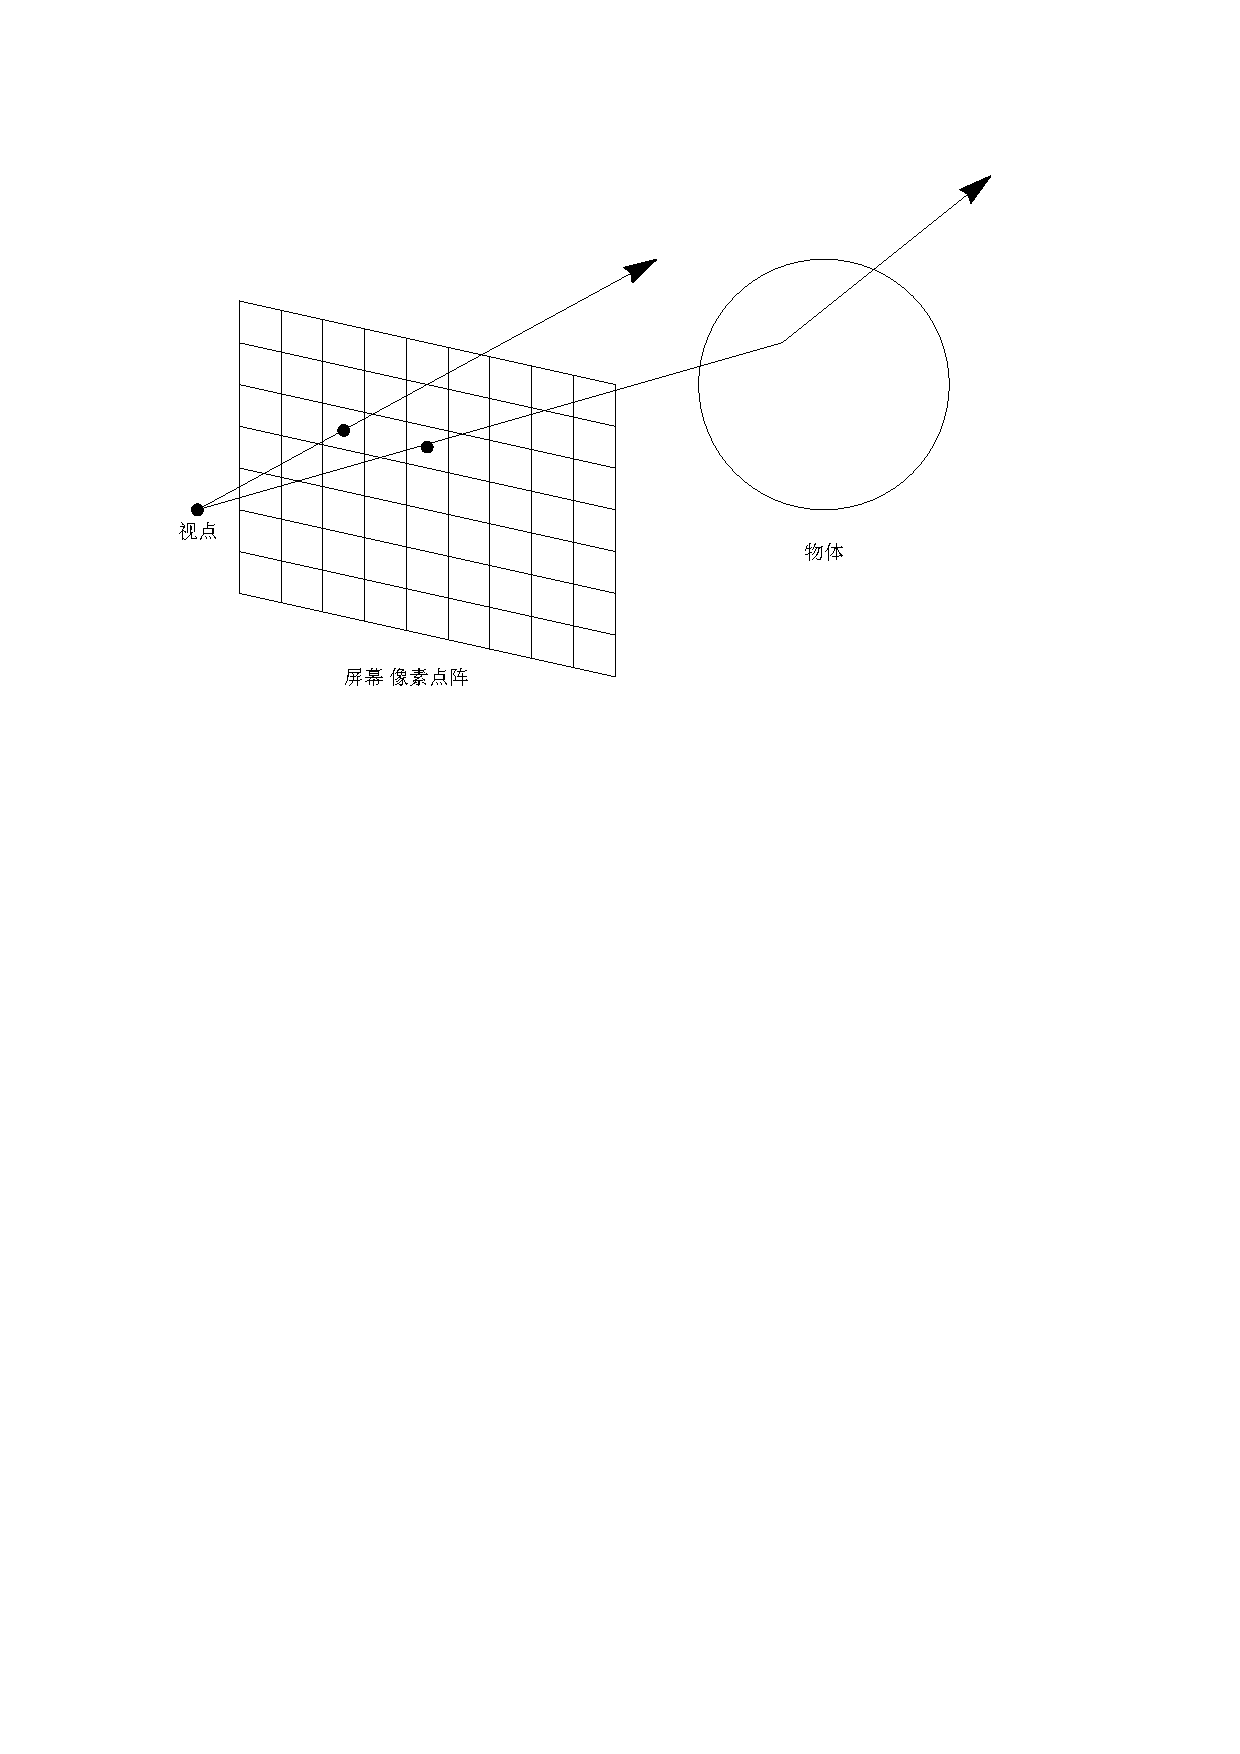
\includegraphics[scale=.55]{fig1.pdf}
\caption{光线追踪基本示意图}
\end{figure}

如图1,通过计算光路上颜色衰减和叠加,即可基本确定每一像素的颜色.

\subsection{\hei 框架}
使用C++实现完整的空间向量类,包括相交检测、计算光线反射与折射.对反射和折射后的光线递归计算颜色再叠加起来即可算得原光线颜色.(若光线未遇到物体则可返回背景色)

在递归的过程中,光亮会不断衰减.因此可以限制迭代的深度或者光亮小于特定值时停止迭代.

将对应于每一像素的光线颜色绘制到图片文件的相应坐标,最后输出绘制所得图像.

基本 rayColor() 递归算法伪代码如下:

\newpage

\begin{algorithm}
  \SetAlgorithmName{\hei 算法}
  \SetAlgoLined
  \text{{\hei 输入:}光线发出位置向量和方向向量}
  \text{{\hei 输出:}反向光颜色}

  {\bf function} rayColor()
  \BlankLine
  
  \eIf{no intersection with any object}{
      \Return{background color}\;
  }{
     {\it obj} $\leftarrow$ find nearest object from the ray\;
     {\it reflect ray} $\leftarrow$ calculate reflect ray with {\it obj}\;
     {\it refract ray} $\leftarrow$ calculate refract ray with {\it obj}\;
     {\it main color} $\leftarrow$ the radiance of {\it obj}\;
	{\it reflect color} $\leftarrow$ rayColor({\it reflect ray})\;
	{\it refract color} $\leftarrow$ rayColor({\it refract ray})\;
     \Return mix({\it main color, reflect color, refract color})\;
  }
   \caption{\hei 光线追踪递归框架}
\end{algorithm}

\section{\hei 初步实现}
对于任意几何体,都需要建立特定函数$f(\mathbf{x})$。自变量$\mathbf{x}$表示空间点的坐标,函数
\begin{equation}
f(x)=
\begin{cases}  -1 & \text{点} \mathbf{x} \text{在几何体外部}\\ 0 & \text{点} \mathbf{x} \text{在几何体表面上}\\ 1 & \text{点} \mathbf{x} \text{在几何体内部}\end{cases}
\end{equation}

\subsection{\hei 计算交点}
复杂几何体都可以近似划分为基本几何体,一般只需要实现光线与球体或平面求交.

光线上的点坐标(以向量表示)可以写为

\begin{equation}\mathbf{p}=\mathbf{s}+t\mathbf{d}\end{equation}

其中$\textbf{s},\textbf{d}$分别是起始点坐标和方向向量.

因此交点可以表示为方程

\begin{equation}f(\mathbf{p}=\mathbf{s}+t\mathbf{d})=0\end{equation}

解出$t$值即可。

\subsubsection{\hei 球体}

球面方程为

\begin{equation}
|\mathbf{p}-\mathbf{c}|=r
\end{equation}

$\mathbf{p}$为(2)式中坐标向量。此时$$f(\mathbf{p})=\sgn(r-|\mathbf{p}-\mathbf{c}|)=0$$

解出$t$值即可。

\subsubsection{\hei 平面}

设平面法向量的坐标为$\mathbf{c}$,法向量方向为$\mathbf{N}$,则有以下方程

\begin{equation}
(\mathbf{p}-\mathbf{c})\mathbf{N}=\mathbf{0}
\end{equation}

同理也可解出交点位置.

\subsubsection{\hei 其他几何体}
可以将复杂曲面划分为许多个小平面(或三角形)的近似.因此将复杂问题化归为光线与空间内多边形求交点.

首先求出光线与多边形所在平面的交点,将此交点的空间坐标向量与该平面的两个基向量相乘即可得到其对应于此平面的二维坐标.

判断平面上点与多边形的位置关系可以使用经典的射线法.

\subsection{\hei 反射光线}
由反射定律,入射光线与反射光线、法线共面,且两条光线关于法线对称.以上讨论的几种基本情况,法线向量$\mathbf{N}$是易求得的.由几何关系可知

\begin{equation}
\mathbf{d'}-\mathbf{d}=2\mathbf{N}
\end{equation}

其中$\mathbf{d'}$是反射光线,故可直接求得.

\subsection{\hei 折射光线}
首先通过折射定律判断是否存在折射,如有则求出折射角.将入射光线、折射光线、法线向量平移拼为三角形,由正余弦定理即可求出折射光线向量.

\subsection{\hei 光照表现}
假设入射光线为$\mathbf{d}$,反射光线为$\mathbf{d'}$,入射点和光源的连线向量为$\mathbf{l}$,那么此处光亮可以定义为\footnote{根据亮度公式可近似推导}

\begin{equation}
k=\cos{<\mathbf{d'},\mathbf{l}>}=\frac{\mathbf{d'l}}{\mathbf{\|d'\|\|l\|}}
\end{equation}

此处反射颜色是原反射颜色乘以$k$之后的值.

\subsection{\hei 颜色}
与传统255色不同,这里颜色使用标准的全值域RGB模型,会更便于计算。将颜色表示为向量$(r,g,b)$,其中$r,g,b$均为0到1之间的实数\footnote{一般的,近似认为三原色光模式为线性且无偏移}.

\subsubsection{\hei 光照颜色}
RGB值为$\mathbf{c_1}$的光线照射到RGB值为$\mathbf{c_2}$的物体上,反射或折射后的颜色为$\mathbf{c_1}\bigotimes\mathbf{c_2}$,$\bigotimes $为笛卡尔积.

\subsubsection{\hei 叠加颜色}
RGB值为$\mathbf{c_1}$的光线和RGB值为$\mathbf{c_2}$的光线叠加后颜色为$\mathbf{c_1}\bigoplus\mathbf{c_2}$,$\bigoplus $为笛卡尔和.叠加后大于1的$r,g,b$值直接赋为1.

\subsubsection{\hei 颜色衰减}
RGB值为$\mathbf{c}$的光线照射在衰减度为$k$的材质表面后,颜色表现为$k\mathbf{c}$.

\subsection{\hei 物体属性}
\subsubsection{\hei 反射比例(reflect)}
表示与物体相交后,有多少比例的光线产生了反射。
\subsubsection{\hei 折射比例(refract)}
表示与物体相交后,有多少比例的光线产生了折射。

\subsection{\hei 初步算法演示}
应用了光源、球面、反射、漫反射、颜色叠加的基本光线追踪模型,效果如右图所示:

\newpage

\begin{figure}[!ht]
\centering
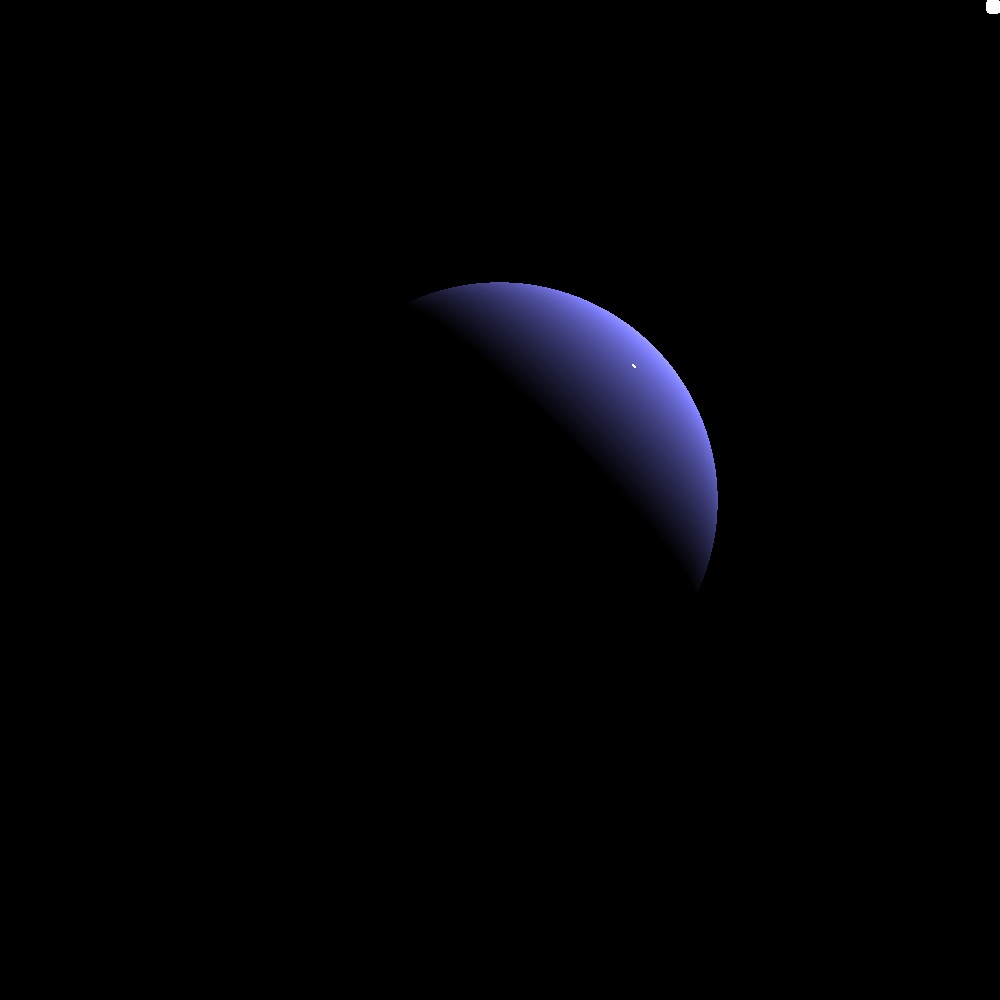
\includegraphics[scale=.2]{fig2.jpg}
\caption{初步算法效果}
\end{figure}

\section{\hei Phong 光照模型}
\subsection{\hei 原理}

为了提供更为真实的渲染效果,Bùi Tuòng Phong 发明了 Phong 着色法。这种方法将漫反射(diffuse reflection)和正反射(specular reflection)叠加在一起,并给正反射加以高光,使得“光晕”效果更明显。

使用Phong着色法需要给物体添加许多额外的物理参数:
\subsection{Phong 模型中的物体属性}
\subsubsection{\hei 漫反射亮度(diffuse)}
表示漫反射光的衰减比例。
\subsubsection{\hei 反射亮度(specular)}
表示正反射光的高光比例。

\subsection{\hei 效果对比图}
\newpage

\begin{figure}[ht]
\centering
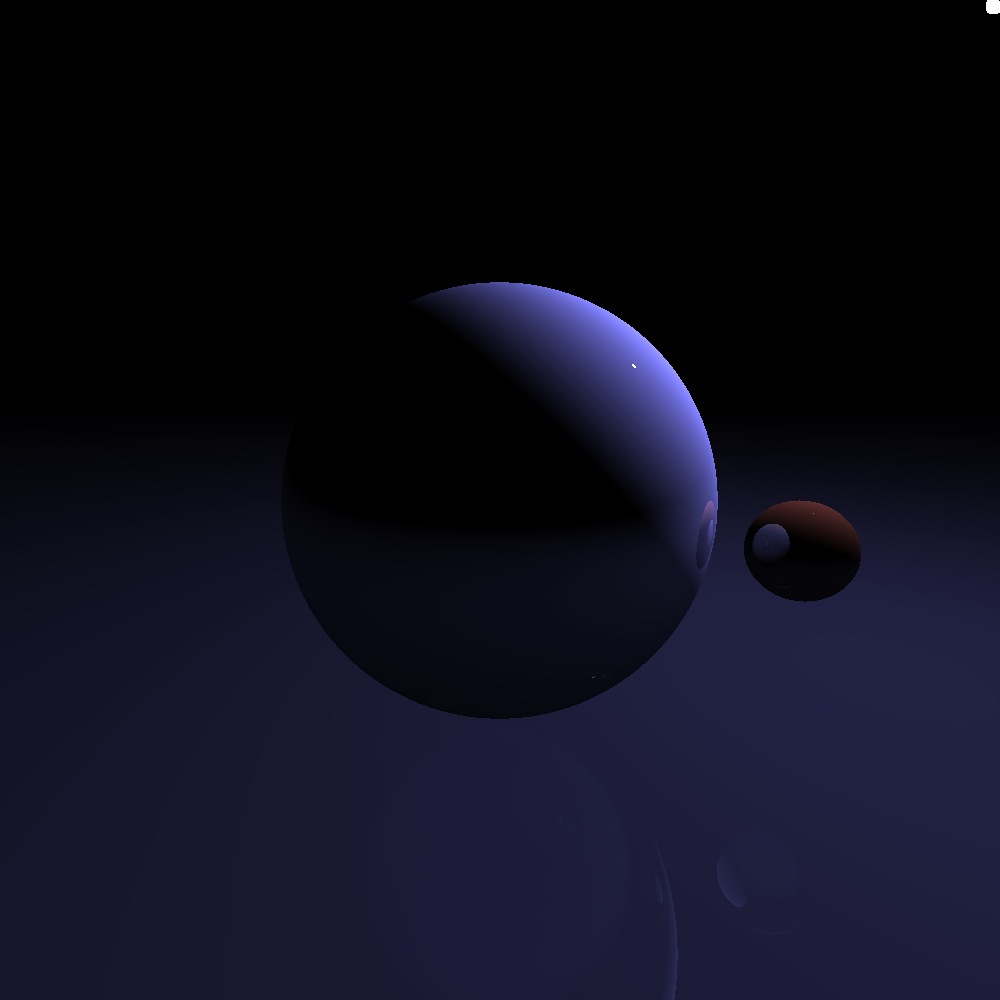
\includegraphics[scale=.2]{fig3.jpg}
\caption{球面及平面反射效果(普通)}
\end{figure}

\subsection{\hei 参数}
“光晕”在越接近正反射处表现得越明显,因此高光函数应选取一个基于夹角余弦值的单调、且剧烈变化的函数。有很多种模拟方法,上图取了额外高光系数
\begin{equation}
s=\cos^{50}{\theta}
\end{equation}
此时物体的表现光由以下组成
\begin{align*}
 &obj.reflect * obj.specular *\cos^{50}{\theta}specularColor\\
 +&obj.reflect * obj.diffuse * diffuseColor\\
 +&obj.refract * refractColor
\end{align*}

\section{\hei 阴影}
阴影和高光一样,也是让渲染增强真实感不可缺少的元素。
\subsection{\hei 计算方法}
将入射点和光源连线,若与物体相交则可判断此处有阴影。

若判断有阴影,则将$obj.reflect,obj.refract$两个参数乘上一个小于$1$的倍数,以产生变暗效果。这里取值$shadowRate=0.4$。

\newpage
\begin{figure}[ht]
\centering
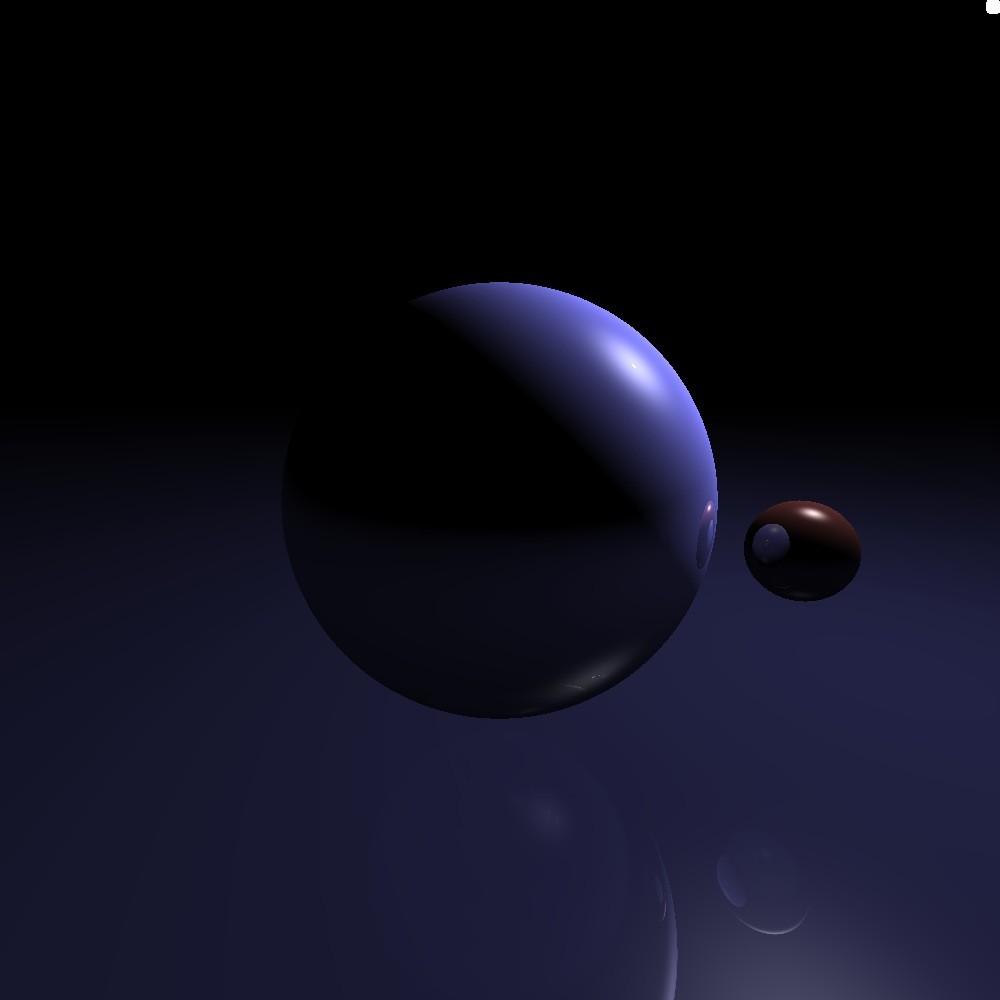
\includegraphics[scale=.2]{fig4.jpg}
\caption{球面及平面反射效果(Phong着色)}
\end{figure}

\subsection{\hei 阴影效果}
\begin{figure}[ht]
\centering
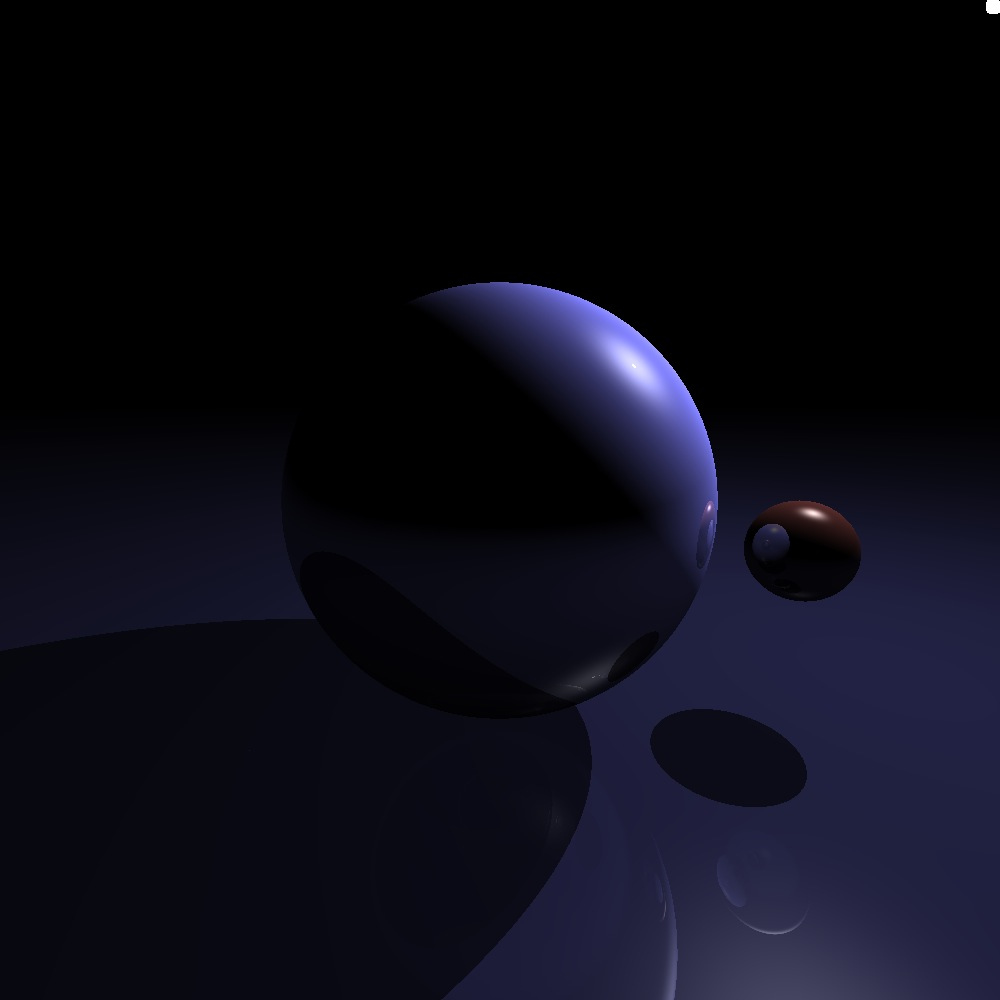
\includegraphics[scale=.2]{fig5.jpg}
\caption{普通阴影}
\end{figure}

\newpage

\subsection{\hei 软阴影和漫反射}
上面产生的阴影,边缘太过尖锐,没有现实中阴影的平滑。软阴影有两种常见渲染方法。
\subsubsection{\hei 采样}
任何物体都不等价于一个质点,光源亦如此。光源放大来看就是一个球体,因此阴影边缘的一个点可能被部分光源照到,那么它就介于阴影和非阴影之间。有一种思路是计算被光照的比例,但难以实现。目前被广泛应用的方法是“采样”。

我们随机在光源球体中取若干个点,并每次将光源定于其中一点,计算阴影。这样计算若干次,每一次由于光源位置稍有不同,故阴影也不同。将这些结果叠加起来,根据概率知识,很容易发现当取点数量达到一定时,叠加起来的阴影越接近真实。

\subsubsection{\hei 蒙特卡罗算法}
蒙特卡罗算法是一大类随机算法的统称,也是另一种接近真实的渲染方法。在现实中不存在绝对平滑的物体,所以不存在正反射。利用这一点,可以在每一次计算反射光的时候随机偏离一个角度。如此随机很多次,再将颜色平均起来就得到这一点的颜色。蒙特卡罗算法既可以模拟计算漫反射,也可以计算软阴影。

给物体添加附加属性“粗糙度”,代表这个随机角的范围。越粗糙的物体表面随机角越大。

\subsubsection{\hei 软阴影和漫反射效果}
\begin{figure}[ht]
\centering
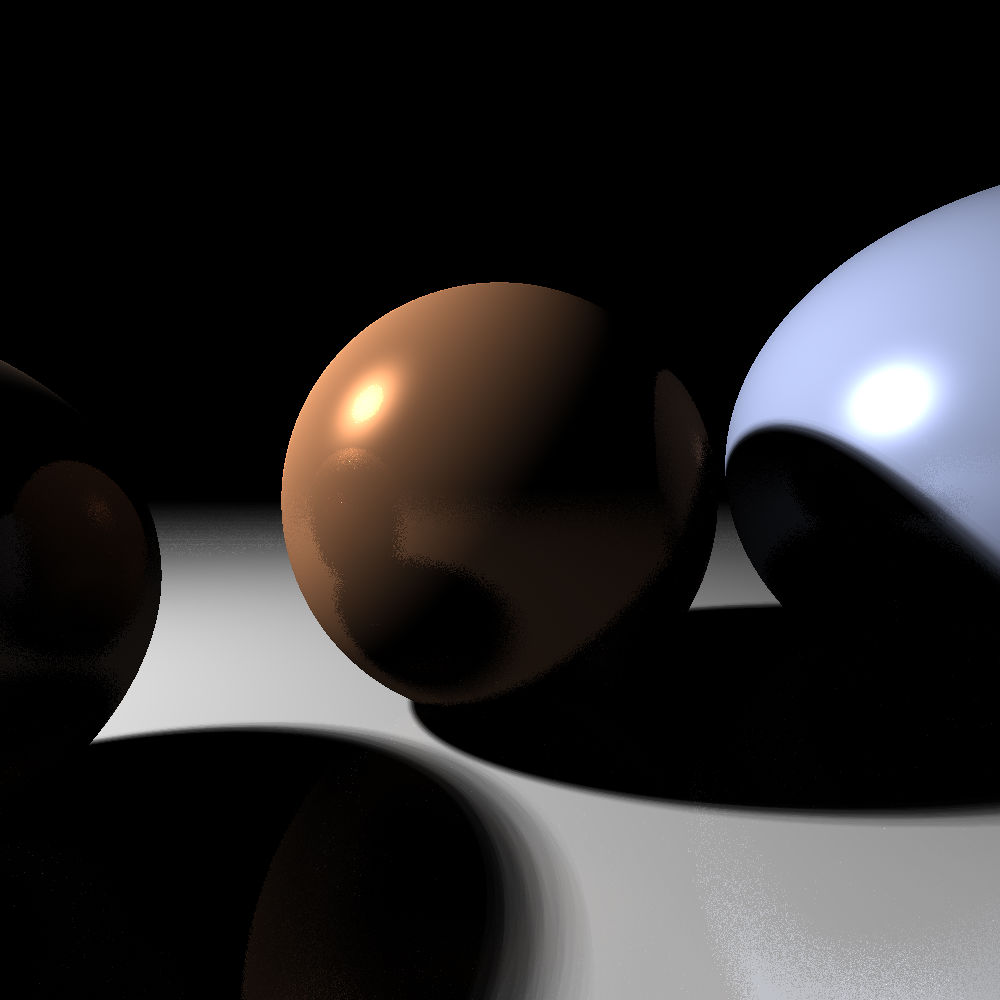
\includegraphics[scale=.18]{fig6.jpg}
\caption{采样与蒙特卡罗算法结合}
\end{figure}

\section{\hei 镜头}
观察发现,靠近画面边缘的球体显示为椭球。这是由于屏幕以斜面截取视线,即所谓的广角镜头。我们可以通过调整屏幕的形状(将平面映射到一个球面上),或者在镜头前加一个透镜。

同一场景,调整镜头前后对比如下:
\begin{figure}[ht]
\centering
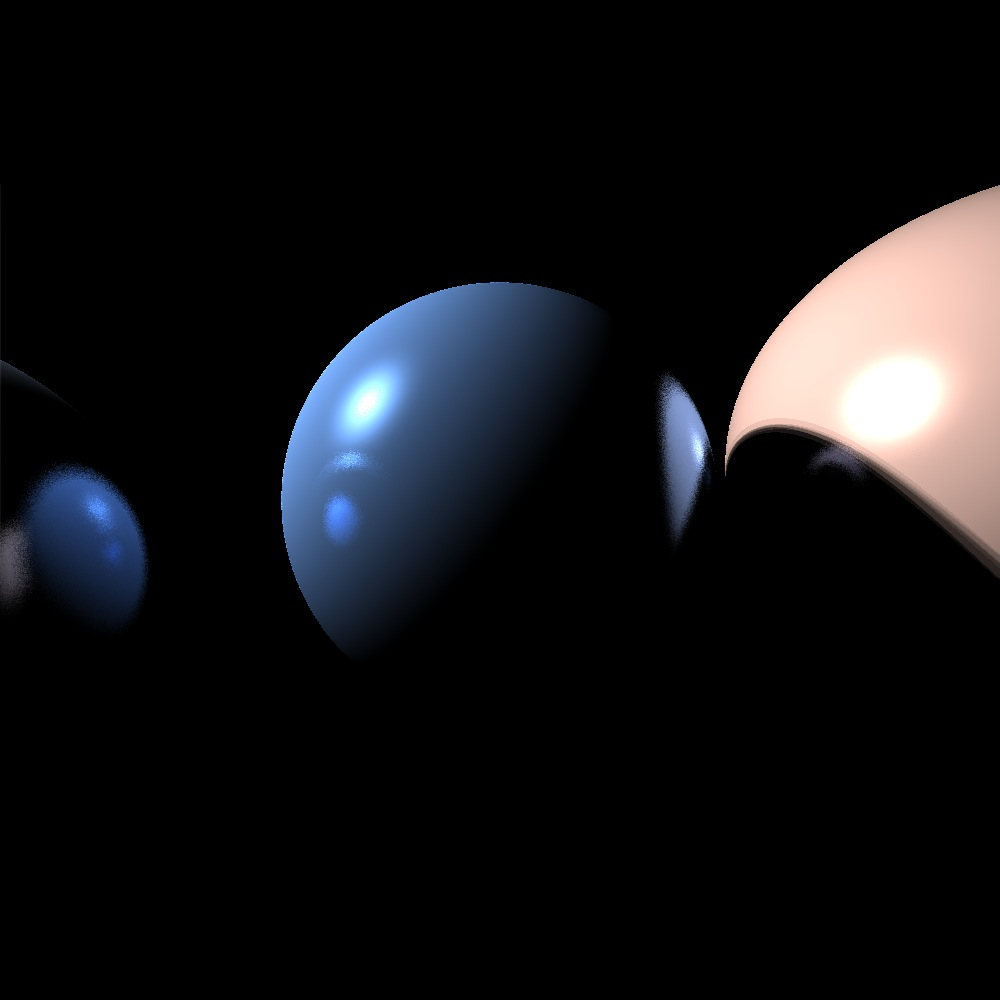
\includegraphics[scale=.2]{fig7.jpg}
\caption{广角镜头}
\end{figure}
\begin{figure}[ht]
\centering
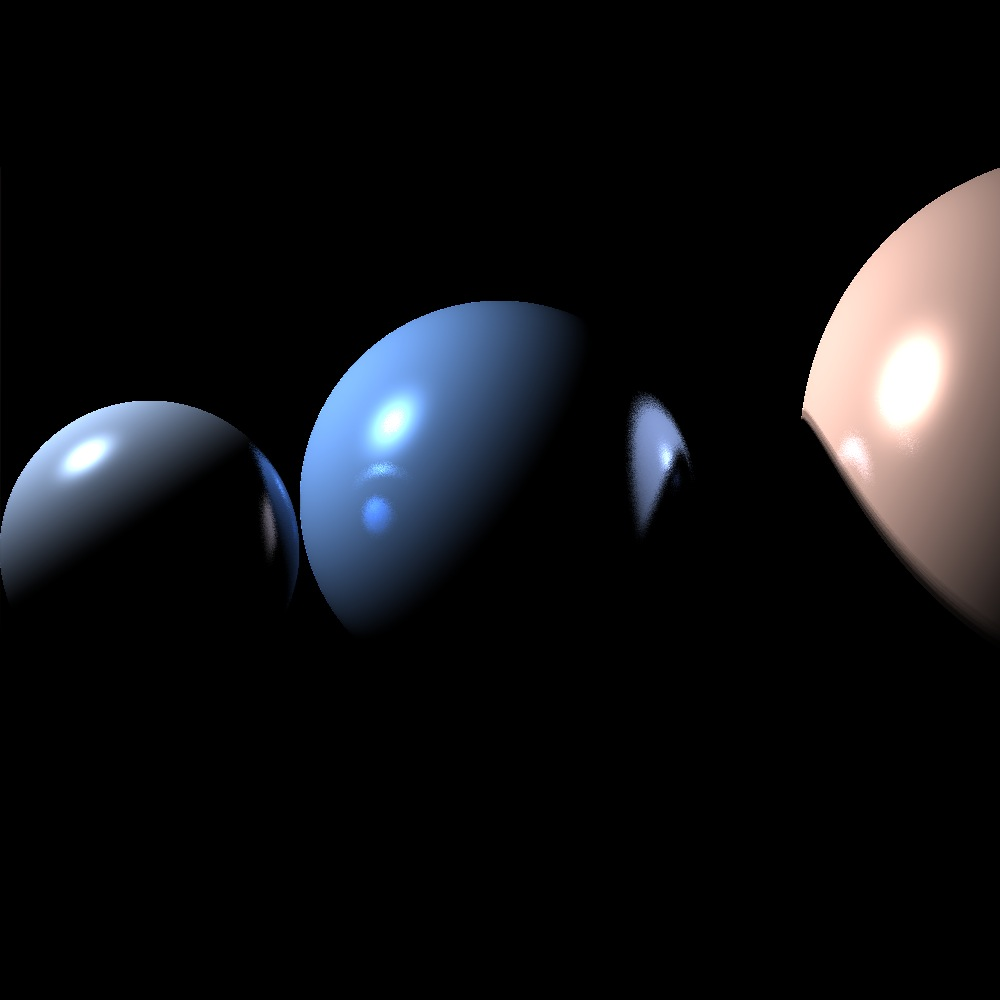
\includegraphics[scale=.2]{fig8.jpg}
\caption{鱼眼镜头}
\end{figure}

\section{\hei 纹理}
通过照射点的三维坐标,可以还原出这个点对于此物体的坐标,基于此就能给物体加上纹理。例如对于平面有

\begin{equation}
\mathbf{x'}=\mathbf{nx}
\end{equation}

其中$\mathbf{n}$是平面的基向量,$\mathbf{x}$是点的三维坐标,$\mathbf{x'}$是点相对于平面的坐标。

\subsection{\hei 改进后的光线追踪效果图}
再对物体的各种参数进行微调,给平面添加纹理后得到效果图如下。
\begin{figure}[ht]
\centering
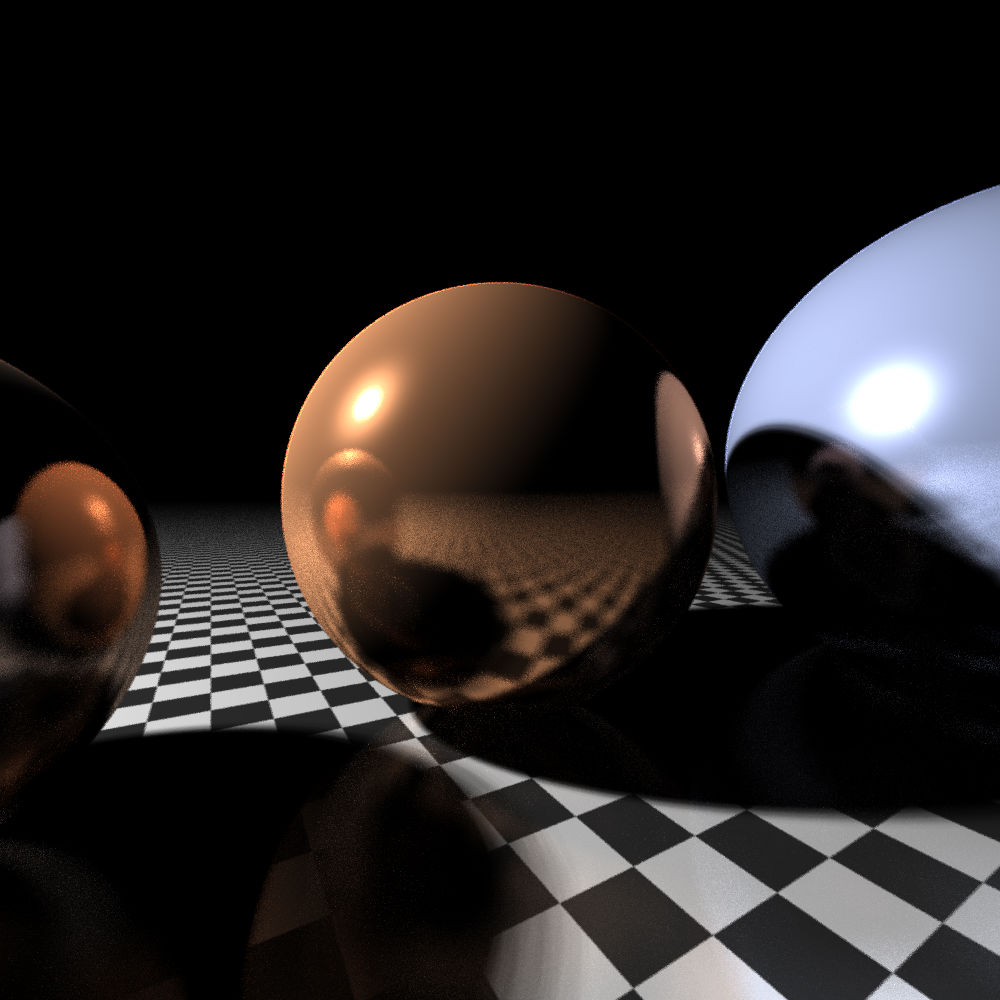
\includegraphics[scale=.2]{fig9.jpg}
\caption{添加纹理后的效果}
\end{figure}

类似的,球面映射也可以通过极坐标(确定经纬度)来计算。

\section{\hei 折射}
光线折射遵循斯涅耳定律
\begin{equation}
\frac{\sin{\theta_1}}{\sin{\theta_2}}=\frac{n_2}{n_1}
\end{equation}

其中$\theta_1,\theta_2$分别为入射角、折射角,$n_1,n_2$表示两种材质的折射率。

\subsection{\hei 计算折射光线}
通过常规解方程法计算折射光线太过繁琐。因为向量之间便于计算夹角,可以通过光学几何关系来确定折射光线。

\begin{figure}[ht]
\centering
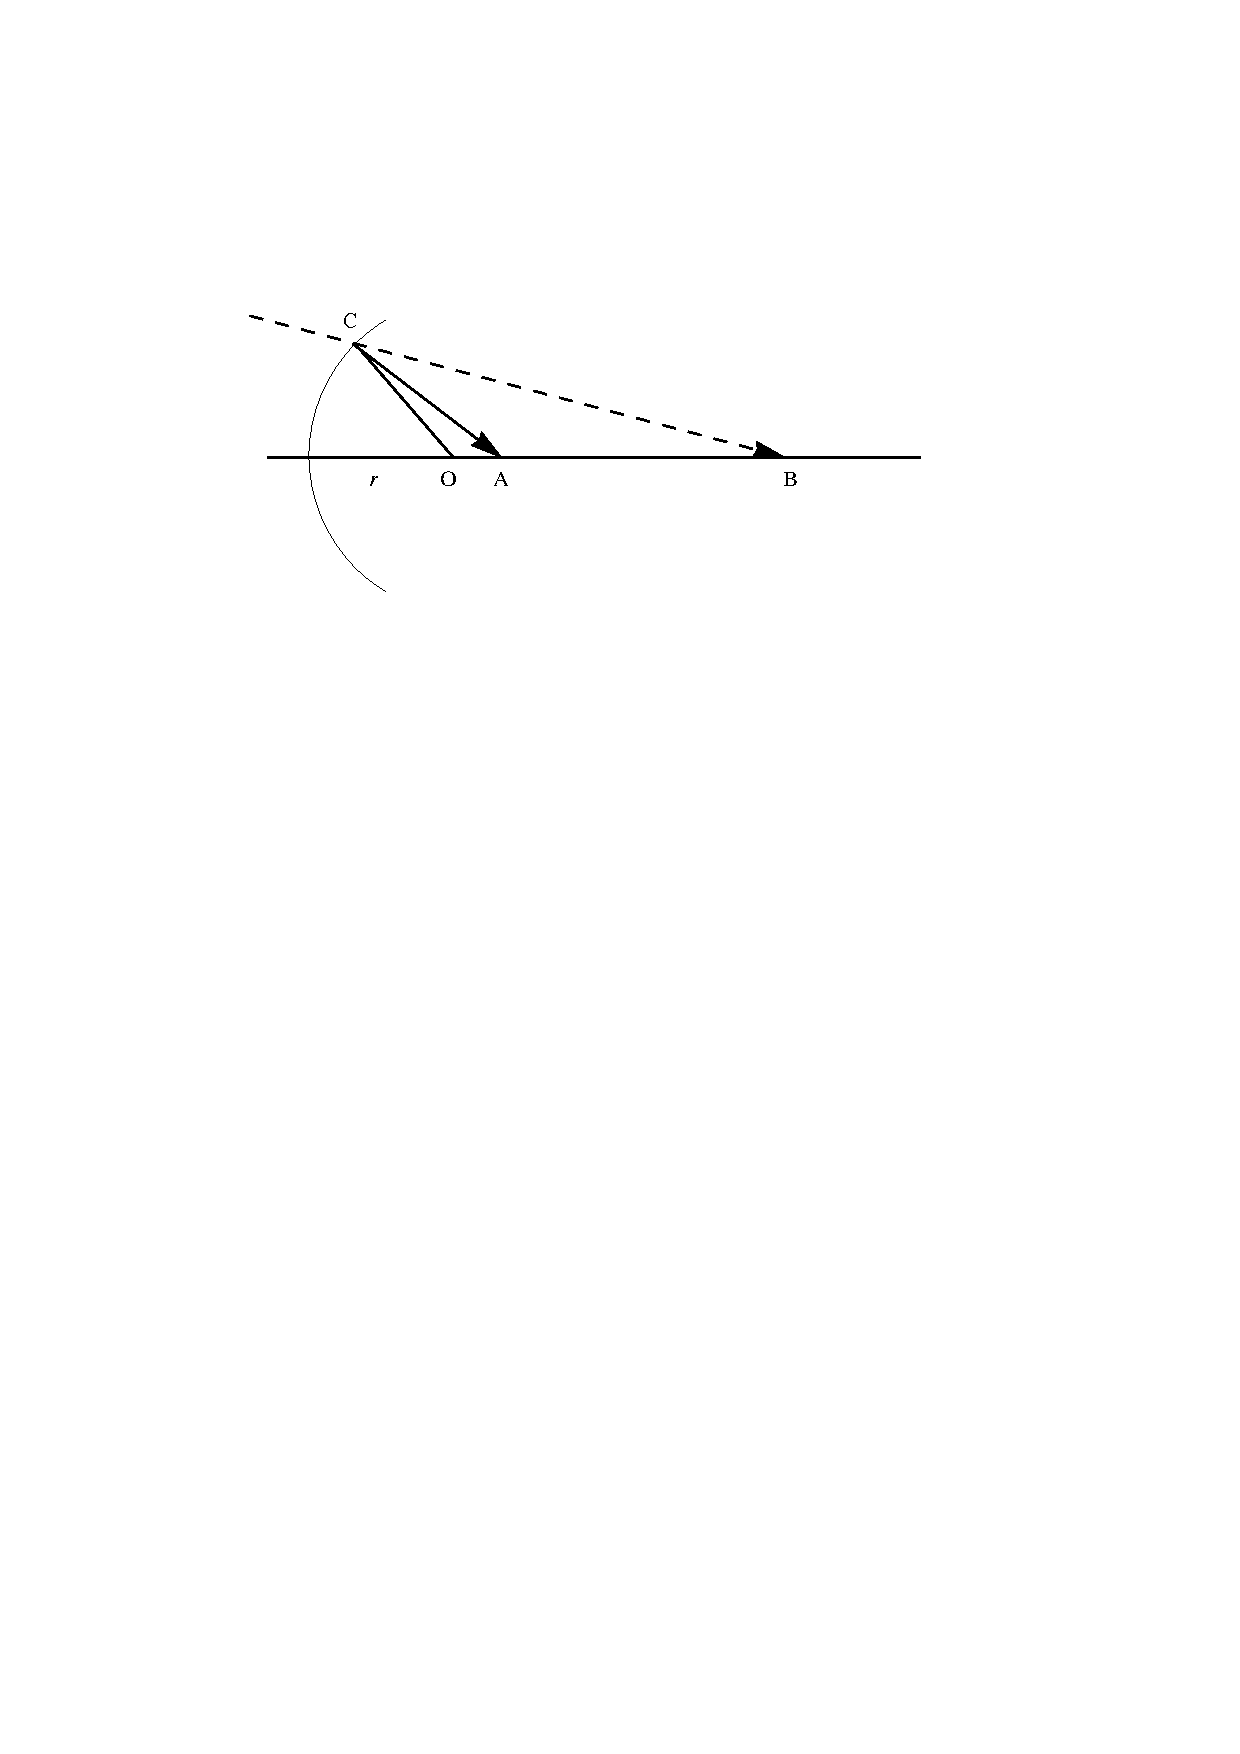
\includegraphics[scale=0.6]{fig10.pdf}
\caption{计算折射光线}
\end{figure}

\end{document}